\begin{figure}
	\centering
	\begin{subfigure}{0.4\textwidth}
		\centering
		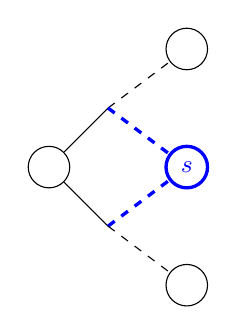
\begin{tikzpicture}[
			wide/.style={line width=4pt}, every node/.style={circle,draw,minimum size=15}, scale=.25]

			\node (root) at (-6,0) {};

			\coordinate (s1) at (-3, 3) {};
			\coordinate (s2) at (-3, -3) {};

			\node  (s3) at (1, 6) {};
			\node[blue, very thick]  (s4) at (1, 0) {};
			\node  (s5) at (1, -6) {};

			\draw (root) -- (s1);
			\draw (root) -- (s2);

			\draw[dashed] (s1) -- (s3);
			\draw[blue, dashed,very thick]  (s1) -- (s4);

			\draw[blue, dashed,very thick]  (s2) -- (s4);
			\draw[dashed]  (s2) -- (s5);

			\node[color=blue, draw=none,fill=none] (s-label) at (s4) {\small$s$};

		\end{tikzpicture}\label{subfig:dag}
	\end{subfigure}
	\hfil
	\begin{subfigure}{0.4\textwidth}
		\centering
		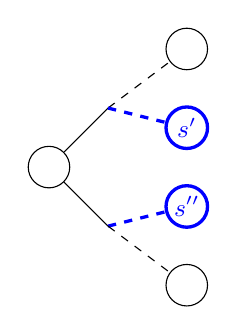
\begin{tikzpicture}[
			wide/.style={line width=4pt}, every node/.style={circle,draw,minimum size=15}, scale=.25]

			\node (root) at (-6,0) {};

			\coordinate (s1) at (-3, 3) {};
			\coordinate (s2) at (-3, -3) {};

			\node  (s3) at (1, 6) {};
			\node[blue,very thick] (s4a) at (1, 2) {};
			\node[blue,very thick]  (s4b) at (1, -2) {};
			\node  (s5) at (1, -6) {};

			\draw (root) -- (s1);
			\draw (root) -- (s2);

			\draw[dashed] (s1) -- (s3);
			\draw[blue, dashed,very thick]  (s1) -- (s4a);

			\draw[blue, dashed,very thick] (s2) -- (s4b);
			\draw[dashed]  (s2) -- (s5);

			\node[color=blue, draw=none,fill=none] (sa-label) at (s4a) {\small$s'$};
			\node[color=blue, draw=none,fill=none] (sb-label) at (s4b) {\small$s''$};

		\end{tikzpicture}\label{subfig:treeified}
	\end{subfigure}
	\caption{
		Converting a DAG structure to a tree, such that the history so far is fully encoded in the current state.
		The state $s$ is split into states $s'$ and $s''$, depending on their parent.
		
	}
\end{figure}
